\documentclass[11pt,a4paper]{article}
\usepackage[margin=25mm,headheight=14pt]{geometry}
\usepackage{amsmath,amssymb}
\usepackage{booktabs,longtable,array}
\usepackage{calc}
\usepackage{graphicx}
\graphicspath{{../}{}}
\usepackage[font=small,labelfont=bf,labelsep=period]{caption}
\usepackage{microtype}
\microtypesetup{expansion=false}
\usepackage[hidelinks]{hyperref}
\usepackage{etoolbox}
\usepackage{setspace}
\setstretch{1.16}
\setcounter{secnumdepth}{0}
\newcounter{none}
\setlength{\parindent}{15pt}
\setlength{\parskip}{0pt}
\setlength{\emergencystretch}{2em}
\sloppy
\setlength{\tabcolsep}{4pt}
\renewcommand{\arraystretch}{1.18}
\providecommand{\tightlist}{\setlength{\itemsep}{0pt}\setlength{\parskip}{0pt}}
\setlength{\LTleft}{\fill}
\setlength{\LTright}{\fill}
\AtBeginEnvironment{longtable}{\small\setlength{\tabcolsep}{3.2pt}\renewcommand{\arraystretch}{1.14}}
\AtBeginEnvironment{figure}{\centering\captionsetup{skip=7pt}}
\newcommand{\pandocbounded}[1]{\resizebox{\linewidth}{!}{#1}}
\newcommand{\FloatBarrier}{\clearpage}
\makeatletter
\renewcommand{\fps@figure}{htbp}
\makeatother
\title{Auditing constrained geospatial allocation under annual land-cover product uncertainty}
\author{Ning Zhou\\[3pt]\normalsize Beijing Freedo Technology Co., Ltd.\\[-1pt]\normalsize Corresponding author: Ning Zhou (\texttt{zhouning@freedotech.com})}
\date{}
\begin{document}
\maketitle
\section{Geospatial Kernel: a state--action--constraint core for urban land-cover planning}\label{geospatial-kernel-a-stateactionconstraint-core-for-urban-land-cover-planning}

\textbf{An Abu Dhabi benchmark with conditional multi-year scenario analysis}

\textbf{Author:} Ning Zhou\\
\textbf{Affiliation:} Beijing Freedo Technology Co., Ltd.\\
\textbf{Corresponding author:} Ning Zhou

This study is not an official Abu Dhabi planning forecast. Correspondence: Ning Zhou, Beijing Freedo Technology Co., Ltd.

\subsection{Abstract}\label{abstract}

Urban land-change models test how development demand may be distributed across space. Their planning value depends on explicit actions, hard constraints and consistent multi-year state transitions. We examine Geospatial Kernel, the algorithmic core of a Geospatial World Model, as an auditable state--action--constraint transition system for urban land-cover allocation. The Abu Dhabi benchmark specifies annual public land-cover products from 2017--2024, a 100-m grid, three computational seeds, destination-correct multi-class change Figure of Merit, persistence and minimum-change controls, spatial-block bootstrap intervals, and a frozen planning objective set spanning accessibility, compactness, fragmentation and vegetation balance. The implementation contribution is an inspectable proposal--projection--writeback execution boundary with fail-closed data and output audits. The public benchmark bundle, model source, checkpoints, historical prediction rasters, planning rasters, vector change packages and mechanism-control report are released with the repository and addressed by a reproducibility manifest. The resulting rankings are conditional pipeline comparisons, not claims of intrinsic learner superiority or official Abu Dhabi forecasting. The benchmark keeps public land-cover stress tests separate from authoritative statutory land use.

\subsection{Highlights}\label{highlights}

\begin{itemize}
\tightlist
\item
  Geospatial Kernel separates transition proposals from constrained admission.
\item
  Typed state--action--constraint traces make recursive updates auditable.
\item
  Spatial-block uncertainty and paired model contrasts are prespecified.
\item
  Four planning dimensions are reported without a weighted composite score.
\item
  Public-data scenarios are stress tests, not statutory Abu Dhabi forecasts.
\end{itemize}

\subsection{Keywords}\label{keywords}

Geospatial World Model; land-cover change; constrained allocation; cellular automata; Abu Dhabi; scenario planning

\subsection{Introduction}\label{introduction}

Land-cover change is a spatial process. Development demand is expressed as a quantity, but its consequences depend on where each new cell is placed relative to roads, existing built areas, ecological features and other land-cover classes. This coupling matters for urban planning because two maps with the same total built area can imply very different infrastructure requirements and environmental pressures. Cellular-automata and suitability-based models have long provided a way to distribute land demand across a map, including CLUE-S, SLEUTH, Dinamica EGO, FLUS, local-attribute urban CA models and more recent patch-generating or deep-learning CA models (Verburg et al., 2002; Silva and Clarke, 2002; Soares-Filho et al., 2002; Lau and Kam, 2005; Liu et al., 2017; Liang et al., 2021). Global Earth-observation products now make it possible to construct annual, spatially aligned inputs for cities that lack a harmonized local data archive (Brown et al., 2022; Gorelick et al., 2017).

Validation studies have also shown that agreement in unchanged cells can mask poor allocation of actual change. Quantity and allocation disagreement, destination-specific transition scores and explicit calibration/validation protocols are therefore preferable to a single overall-accuracy number (Pontius et al., 2008; Pontius and Millones, 2011; van Vliet et al., 2011, 2016). This distinction is central here because the benchmark uses noisy annual labels and tests both one-step allocation and recursive rollout.

The main technical difficulty is not producing another categorical raster. It is keeping the semantics of a planning action separate from the learned transition tendency. A model may predict that a cell is likely to become built, yet the resulting map can still violate a water exclusion, miss the requested class totals or become inconsistent when the next year is simulated from the model's own output. These failure modes are particularly important when the model is used to compare scenarios rather than to reproduce one observed transition. Latent-dynamics approaches such as GeoFM-LDN can represent continuous geospatial state and condition transitions on demand, whereas traditional ANN-plus-cellular-automata systems such as GeoSOS-FLUS combine suitability with explicit neighbourhood evolution. Neither design, by itself, guarantees that action semantics, hard constraints, state persistence and evidence provenance are visible at the same execution boundary.

We address this systems problem by studying Geospatial Kernel, the core transition layer of a Geospatial World Model (GWM). The Kernel represents one simulation step as a typed state, a typed action, a transition proposal, a constraint projection and a state writeback. The learned proposal remains domain-specific; the runtime contract is domain-neutral. For Abu Dhabi land-cover planning, the proposal is a six-class probability cube, and the projection allocates only mutable cells until the action's feasible class totals are reached. This separation makes the planning operation inspectable: a reviewer can distinguish what the transition model preferred from what the constraints admitted.

We evaluate this design in a controlled public-data benchmark rather than treating the benchmark as an official data release. All candidates consume the same 100-m grid, common valid mask, annual class-count actions, hard exclusions and evaluator. The historical track uses observed target counts to isolate spatial allocation skill from demand error. The planning track starts from the observed 2024 state and applies three planner-supplied actions: moderate growth, green-priority growth and high outward growth. Abu Dhabi Plan 2030 provides an institutional planning context for discussing urban structure, but the numerical actions in this benchmark are not calibrated to that plan or to an official population forecast (Abu Dhabi Urban Planning Council, 2007). We ask four questions: whether the Kernel execution contract is auditable, whether its allocation skill is competitive, whether it produces feasible and spatially distinct allocations and which conclusions survive label and parameter sensitivity.

The paper makes three bounded contributions. First, it gives a concrete state--action--constraint formulation for using a geospatial kernel as an algorithmic core rather than as an opaque end-to-end predictor. Second, it reports a multi-horizon pipeline comparison with GeoSOS-FLUS and GeoFM-LDN, including a case in which the Kernel does not win, while making the input imbalance explicit. Third, it turns the future maps into explicit stress-test artefacts, including cumulative rasters and vectorized transition footprints, while preserving the distinction between public-data land cover and authoritative legal land use.

\subsection{Methods}\label{methods}

\subsubsection{Study boundary, grid and temporal protocol}\label{study-boundary-grid-and-temporal-protocol}

The study boundary is the polygon returned for OpenStreetMap relation R4479763, representing Abu Dhabi city. All rasters were aligned to a canonical 100-m grid in EPSG:32640 with 475 columns and 360 rows. A cell was included when its centre fell within the city polygon and when the common public-data mask indicated valid coverage. The benchmark profile records the source geometry, raster transform, dimensions and SHA-256 hashes. The effective evaluation mask contains 79,726 cells.

The observed sequence contains annual states for 2017--2024. Models were fit using the four transitions 2017→2018, 2018→2019, 2019→2020 and 2020→2021. A 2021→2022 transition was used for validation during model development. The historical test starts from 2022 and evaluates 2023 and 2024 in an open-loop rollout without observed-state writeback. The planning test starts from the observed 2024 state and recursively generates 2025--2031 under each scenario action.

\subsubsection{Public data and class semantics}\label{public-data-and-class-semantics}

Dynamic World V1 provides annual scene-argmax labels and mean top-class probabilities (Brown et al., 2022). The nine Dynamic World labels were crosswalked to six canonical classes: water (source 0), woody vegetation (1), low vegetation (2, 4 and 5), wetland (3), built (6) and bare (7). Source class 8 was excluded. The resulting label is explicitly treated as land cover. No residential, commercial or industrial category is inferred from the raster labels.

Annual 64-dimensional AlphaEarth embeddings were spatially averaged to the canonical grid and locally L2-normalized. Monthly VIIRS night-time-light radiance was averaged by year. Copernicus DEM supplied elevation and a finite-difference slope derivative. OpenStreetMap road geometries were rasterized into distance-to-road and distance-to-major-road surfaces. ESA WorldCover 2021 supplied public water and wetland/mangrove constraint proxies (Zanaga et al., 2022). All dynamic and static layers were checked for exact CRS, transform, width and height agreement.

\subsubsection{Geospatial Kernel state, action and transition proposal}\label{geospatial-kernel-state-action-and-transition-proposal}

Let \(S_t(i)\) denote the six-class state at valid cell \(i\), \(A_t\) the action for the interval \(t\rightarrow t+1\), and \(X_t\) the aligned driver layers. The Kernel separates a proposal from a projection:

\[
Q_t(i,c)=p_\theta\big(c\mid x_i(S_t,X_t)\big),
\qquad
S_{t+1}=\Pi_{\mathcal C,A_t}(Q_t,S_t).
\]

The feature vector \(x_i\) contains 25 values: six one-hot current-class indicators; twelve neighbourhood proportions, comprising 3 × 3 and 7 × 7 windows for each of the six classes; and seven continuous variables, namely normalized row and column coordinates, clipped elevation, clipped slope, log-transformed VIIRS radiance, log distance to roads and log distance to major roads. A histogram gradient-boosting classifier estimates the six-class probability vector. It uses learning rate 0.08, 120 iterations, at most 31 leaf nodes, minimum leaf size 40 and L2 regularization 1.0.

Training samples combine all changed valid cells and a 20\% random sample of stable valid cells in each fit transition. The sample weight is the product of a change emphasis, \(1+5\mathbf{1}(S_t\ne S_{t+1})\), and a confidence factor, \(0.5+\min(r_t,r_{t+1})\), where \(r\) is the Dynamic World mean top probability. The target years 2023 and 2024 are not used during fitting or model selection. Across the three seeds, each fitted model used 71,892--72,202 pixel rows and all six classes.

\subsubsection{Constraint projection and state writeback}\label{constraint-projection-and-state-writeback}

For a mutable source cell \(i\) of class \(s\) and target class \(c\), the base allocation score is

\[
q_{i,s\rightarrow c}=\log p_\theta(c\mid x_i)-\log p_\theta(s\mid x_i)+\lambda\rho^{(7)}_{i,c},
\]

where \(\rho^{(7)}_{i,c}\) is the 7 × 7 fraction of neighbouring cells currently in class \(c\), and \(\lambda=0.35\). The algorithm computes class deficits and excesses from the action's feasible target counts, ranks all admissible source--target candidates by \(q\), and changes cells in descending order until all deficits and excesses are zero. Permanent water and the protected wetland/ecological mask are held fixed. If the counts cannot be satisfied without changing a hard-exclusion cell, the step fails closed rather than silently violating the action.

The projected raster is written as the next \texttt{KernelState}. Every step records a state reference, action evidence, model version, parameter reference, projection status and diagnostic counts. The runtime checks domain identity, source-time consistency and action time advancement. This execution contract is the Geospatial Kernel's algorithmic contribution; the Abu Dhabi adapter supplies the land-cover-specific features, learner and constraint masks.

\subsubsection{Baselines and common evaluator}\label{baselines-and-common-evaluator}

GeoSOS-FLUS was run through the external FLUS console using seven continuous drivers: normalized row and column coordinates, elevation, slope, VIIRS radiance, distance to roads and distance to major roads. Its ANN suitability surface was passed to a cellular-automata allocation stage with the common class totals and public hard mask. The archived run used one 2021 training year, eight ANN hidden neurons, a 3 × 3 CA neighbourhood, neighbourhood strength 1.0, acceleration factor 0.1 and 1,000 iterations. Its frozen transition matrix protected water and wetland but did not prohibit built-to-non-built transitions; this configuration is recorded as a baseline limitation rather than a calibrated Abu Dhabi model. The supplied Mach-O executable cannot be traced to a reproducible upstream release or source commit, so we do not claim bitwise equivalence to the Liu et al.~(2017) FLUS implementation.

GeoFM-LDN (Geospatial Foundation-Model Latent Dynamics Network; the repository's former \texttt{paper58} path identifier) was implemented as a demand-conditioned residual latent-dynamics network on 64-channel AlphaEarth patches. Three 128-channel convolutions use dilation rates 1, 2 and 4, followed by a 1 × 1 projection to a 64-dimensional latent state. A 12-dimensional action vector (origin and target counts for six classes) is encoded by a two-layer MLP and broadcast across the patch before concatenation with the embedding. Group normalization and GELU activations are used in the residual blocks. A scikit-learn logistic-regression decoder maps the predicted latent embedding to six semantic classes. Training uses 64 × 64 patches, batch size 2, eight epochs, AdamW with learning rate \(3\times10^{-4}\) and weight decay \(10^{-4}\); the loss is the weighted sum of cosine embedding loss, 0.5 semantic cross-entropy, 0.1 demand-consistency loss and 0.2 hard-constraint consistency loss. The released checkpoints correspond to seeds 31, 47 and 73 and were trained in August 2026. The default reproduction loads these fixed checkpoints rather than retraining; the runner exposes retraining separately. During allocation, GeoFM-LDN directly calls the Geospatial Kernel \texttt{allocate\_action} routine, so both methods share the same constrained projection and differ primarily in their proposal model. The comparison is therefore a proposal/pipeline comparison, not a comparison of two independent projection architectures. The name describes this benchmark implementation and does not attribute an external publication or performance claim.

The common evaluator computes actual class counts, normalized demand total variation, hard-mask violations, strict multi-class change FoM, binary change FoM, change F1, overall accuracy and macro-F1 for historical runs. The strict FoM counts a hit only when the predicted destination class equals the observed destination class; wrong destination changes are retained in the denominator. It also generates persistence and minimum-change zero controls, spatial-block bootstrap intervals and paired model-difference intervals for strict FoM, overall accuracy and macro-F1. For planning runs it additionally computes ecological conversion, new-built neighbourhood fraction, built component counts, built components per 1,000 valid pixels, a 500-m leapfrog rate, distances to roads and prior built cells, infrastructure proxy distance and built retirement. Pareto membership is calculated only over the frozen four-dimensional set of major-road distance, prior-built distance, built-component density and green-cell gain; the remaining quantities are reported as descriptive diagnostics.

\subsubsection{Scenario actions and uncertainty}\label{scenario-actions-and-uncertainty}

The moderate-growth, green-priority-growth and high-outward-growth actions are stored in the tracked \texttt{planning\_scenarios\_public\_2025\_2031.json} manifest; the legacy \texttt{compact} path identifier is retained only for artifact compatibility. Each action supplies feasible class totals for 2025--2031. The 2031 totals are an explicit extension of the previous annual difference and are not derived from an official population, housing or infrastructure forecast. Future exogenous rasters are held at their 2024 values. The green-priority action is not a water-budget model. Each candidate is run at seeds 31, 47 and 73, and planning tables report arithmetic means and population standard deviations. No p-values are reported because the three seeds describe computational variability, not independent field samples.

\subsubsection{Change polygons and reproducibility}\label{change-polygons-and-reproducibility}

For each model--scenario pair, annual and cumulative differences from the 2024 raster are extracted as changed 100-m cells and dissolved into GeoPackage layers. The public delivery manifest covers 45 ensemble rasters for 2027--2031 and nine vector packages. The audit script reports \texttt{INCOMPLETE\_INPUTS} or \texttt{FAIL} when source rasters, reports or vectors are absent; with the recovered local bundle, the input audit passed all alignment gates (with a Dynamic World label-noise warning) and the output audit passed 276 historical and planning predictions with zero failures. The vector layers preserve raster-cell geometry and should not be interpreted as cadastral parcels.

\subsection{Results}\label{results}

\subsubsection{A common benchmark separates allocation skill from demand assumptions}\label{a-common-benchmark-separates-allocation-skill-from-demand-assumptions}

The benchmark covers the Abu Dhabi city polygon represented by OpenStreetMap relation R4479763. The canonical grid is a 475 × 360 lattice in EPSG:32640 at 100-m resolution. After the common coverage and alignment checks, 79,726 cells were used for scoring. Each cell represents 1 ha. Annual Dynamic World observations from 2017 to 2024 were harmonized to six land-cover classes: water, woody vegetation, low vegetation, wetland, built and bare. AlphaEarth annual embeddings, VIIRS night-time lights, Copernicus DEM derivatives and OpenStreetMap road distances supplied transition drivers. ESA WorldCover and public OpenStreetMap geometries supplied water, wetland and infrastructure exclusion proxies.

The comparison shared the canonical grid, origin states, target actions, hard masks and evaluator, but the public-data run was not information-balanced. GeoSOS-FLUS used seven continuous drivers in its external ANN suitability model, whereas Geospatial Kernel used 25 features including current-class indicators and neighbourhood proportions; GeoFM-LDN used AlphaEarth latent embeddings and the Kernel allocator. We therefore report an unmatched-input pipeline comparison, not evidence that one learner is intrinsically superior. A matched-input FLUS rerun remains necessary for a model-level comparison. The archived FLUS console is a Mach-O arm64 executable whose original source/version cannot be independently rebuilt from this release, so FLUS results are bounded to the supplied Apple-Silicon binary and are not asserted to be bitwise equivalent to an upstream Liu et al.~build. All models used seeds 31, 47 and 73.

The execution trace makes the distinction between proposal and admission explicit. A Kernel step records the source state, action, probability-cube proposal, projected state, model identity, input evidence and next-state reference. The runtime checks that the action advances the source time and that the projected raster becomes the next state. This is the operational meaning of the Kernel in this study: not a claim that all GWM domains share the same learner, but a claim that they can share an auditable execution contract. The shared inputs and execution boundary are summarized in Fig. 1.

\subsubsection{Historical and planning results}\label{historical-and-planning-results}

The historical track uses observed target class totals to isolate spatial allocation from demand estimation. The primary metric is strict multi-class change FoM: a hit requires the predicted destination class to equal the observed destination class, while wrong destination changes remain in the denominator (Pontius et al., 2008). Overall accuracy, macro-F1, change F1 and binary FoM are secondary diagnostics. Uncertainty is estimated with an 8 × 8-pixel spatial-block bootstrap, and model contrasts are computed from the same resampled blocks for each frozen seed. Persistence and random minimum-change allocation are prespecified controls.

The planning track starts from the observed 2024 state and applies three synthetic class-count actions through 2031. Before this recompilation, the objective set was frozen to four non-redundant dimensions: mean distance of new built cells to major roads (accessibility proxy), mean distance to pre-existing built cells (compactness proxy), built components per 1,000 valid cells (fragmentation) and green-cell gain (vegetation-balance direction). Ecological conversion, 500-m leapfrog rate, built retirement and demand error remain descriptive diagnostics because the exact-count projection makes some of them structural zeros or unstable across models. No weighted composite score is used. The choice follows a transparent planning logic: accessibility and proximity to existing development represent infrastructure-efficient urban form, component density penalizes spatial fragmentation, and the opposing vegetation-gain direction prevents a compactness-only objective from defining the frontier. These are measurable public-data proxies rather than claims about welfare, equity or statutory zoning.

The recovered public-data bundle supports a complete re-scoring of the frozen historical rasters and a re-compilation of the 2025--2031 planning rasters. The strict multi-class transition FoM (mean across three seeds) was 0.1256, 0.1961 and 0.1619 for GeoSOS-FLUS, Geospatial Kernel and GeoFM-LDN in 2023, and 0.1782, 0.2529 and 0.2708 in 2024, respectively. Under this unmatched public-data pipeline, Geospatial Kernel had the largest 2023 value, whereas GeoFM-LDN had the largest 2024 value after recursive two-step rollout; no single model dominated both horizons. These rankings are conditional on the different inputs, learners and shared evaluation projection.

\textbf{Table 1 \textbar{} Historical allocation scores.} Values are means across the three frozen computational seeds; the strict multi-class change FoM is the primary metric and the remaining columns are diagnostics. Persistence and random minimum-change are prespecified controls rather than learned models.

{\def\LTcaptype{none} % do not increment counter
\begin{longtable}[]{@{}
  >{\raggedleft\arraybackslash}p{(\linewidth - 10\tabcolsep) * \real{0.1667}}
  >{\raggedleft\arraybackslash}p{(\linewidth - 10\tabcolsep) * \real{0.1667}}
  >{\raggedleft\arraybackslash}p{(\linewidth - 10\tabcolsep) * \real{0.1667}}
  >{\raggedleft\arraybackslash}p{(\linewidth - 10\tabcolsep) * \real{0.1667}}
  >{\raggedleft\arraybackslash}p{(\linewidth - 10\tabcolsep) * \real{0.1667}}
  >{\raggedleft\arraybackslash}p{(\linewidth - 10\tabcolsep) * \real{0.1667}}@{}}
\toprule\noalign{}
\begin{minipage}[b]{\linewidth}\raggedleft
Target year
\end{minipage} & \begin{minipage}[b]{\linewidth}\raggedleft
GeoSOS-FLUS
\end{minipage} & \begin{minipage}[b]{\linewidth}\raggedleft
Geospatial Kernel
\end{minipage} & \begin{minipage}[b]{\linewidth}\raggedleft
GeoFM-LDN
\end{minipage} & \begin{minipage}[b]{\linewidth}\raggedleft
Persistence
\end{minipage} & \begin{minipage}[b]{\linewidth}\raggedleft
Random minimum-change
\end{minipage} \\
\midrule\noalign{}
\endhead
\bottomrule\noalign{}
\endlastfoot
2023 (1-step) & 0.1256 & \textbf{0.1961} & 0.1619 & 0.0000 & 0.0253 \\
2024 (2-step open-loop) & 0.1782 & 0.2529 & \textbf{0.2708} & 0.0000 & 0.0605 \\
\end{longtable}
}

Spatial-block bootstrap model contrasts support these differences. For 2023, Kernel minus FLUS was 0.0703 {[}0.0558, 0.0866{]} and GeoFM-LDN minus Kernel was −0.0341 {[}−0.0479, −0.0209{]}. For 2024, GeoFM-LDN minus Kernel was 0.0177 {[}0.0033, 0.0314{]}. These are conditional pipeline contrasts on public labels, not independent-sample significance tests. The persistence control had higher overall accuracy than every learned candidate (0.9436 in 2023 and 0.8938 in 2024), illustrating why change-specific metrics are necessary. Figure 2 shows the four historical metrics alongside the persistence and random minimum-change controls; bars use three-seed population standard deviations, whereas the paired spatial-block intervals above are the uncertainty summaries used for model contrasts.

The reliability sensitivity is substantially less favourable. Requiring both the origin and target Dynamic World mean top probability to exceed 0.5 leaves strict FoM at 0.000 for all three models in 2023; in 2024 the means are 0.004 for GeoSOS-FLUS, 0.005 for Geospatial Kernel and 0.019 for GeoFM-LDN. This is a label-quality diagnostic, not an independent validation set. Dynamic World also reports built pixels increasing from 9,359 in 2022 to 15,598 in 2024 (67\%), while the median one-year reversion fraction is 0.3611 and the mean fraction of cells below confidence 0.5 is 0.5497. Test-year change counts are approximately twice the training-transition counts. Because the same grid cells recur across years and the Kernel includes coordinate features, a training--test memory effect cannot be excluded; the reported scores should therefore be interpreted as conditional agreement with the public product.

The planning compiler evaluated all nine model--scenario candidates under the frozen balanced objective set. Six candidates---each GeoSOS-FLUS scenario and each Geospatial Kernel scenario---were non-dominated; no GeoFM-LDN candidate was on this conditional frontier. The result should not be read as a model ranking: the frontier is sensitive to public proxy layers, synthetic actions and the declared directions. Geospatial Kernel had lower mean distances to roads and prior built cells than the other candidates, but its built-component density was 2.92--4.28 per 1,000 valid cells, compared with 0.92--1.23 for GeoSOS-FLUS and 3.21--4.35 for GeoFM-LDN. This fragmentation disadvantage is retained rather than hidden by the objective set (Fig. 3). The 2031 majority-vote ensemble L1 demand errors were 8, 44 and 42 pixels for Geospatial Kernel's moderate, green-priority and high-outward scenarios, respectively; the corresponding GeoFM-LDN errors were 1,580, 1,524 and 1,148 pixels and GeoSOS-FLUS errors were 2,504, 2,888 and 2,568 pixels. Seed-level projections meet their feasible class totals, but majority voting can produce a different raster and therefore a non-zero ensemble error. All 276 historical and planning prediction records passed the raster audit, including grid alignment, class validity, outside-mask cleanliness and hard-exclusion checks. The resulting 2031 ensemble rasters and their dissolved cell-change footprints are shown in Fig. 5; they are scenario-conditioned land-cover maps, not parcel boundaries or statutory zoning maps.

\subsubsection{Sensitivity shows a stable but not fully explained neighbourhood contribution}\label{sensitivity-shows-a-stable-but-not-fully-explained-neighbourhood-contribution}

The base Kernel allocation score adds a 7 × 7 target-class neighbourhood fraction with weight 0.35. The existing sensitivity and mechanism artefacts are retained as diagnostic controls; they do not identify a causal effect because the proposal features and allocator both contain spatial context. The neighbourhood term is therefore interpreted as evidence about the execution mechanism, not as an independently estimated planning preference. Figure 4A shows the proposal controls, while Fig. 4B--D reports runtime and planning controls.

\subsubsection{Mechanism controls separate learned proposal from runtime projection}\label{mechanism-controls-separate-learned-proposal-from-runtime-projection}

Mechanism controls separate the learned proposal from runtime projection, hard constraints and recursive writeback. They are not causal policy experiments. Deleting the action reduces mean strict FoM by 0.114 in 2023 and 0.171 in 2024, whereas deleting the hard constraint increases it by 0.014 and 0.011, respectively. The former is expected because the historical task supplies oracle target counts; it shows that much of the measured skill belongs to the action-conditioned allocator rather than to a demand forecast. The latter is an important warning: allowing changes inside the exclusion mask can improve agreement with noisy labels while violating the planning contract. The controls therefore support an execution-level interpretation but do not prove that either component causes an urban outcome.

\subsection{Discussion}\label{discussion}

This study positions Geospatial Kernel as a candidate execution layer for constrained spatial reasoning. The defensible contribution is that a transition proposal and a planning admission rule can be represented and inspected separately. Under the unmatched public-data pipeline, Geospatial Kernel has the largest strict transition FoM at the one-step horizon, while GeoFM-LDN has the largest value after recursive two-step rollout. We therefore avoid a universal superiority claim and treat the planning frontier as conditional on the frozen public-data proxy objectives.

The proposed mechanism is explicit: the score compares the learned probability of a target class with that of the current class and adds local support from the target-class neighbourhood. The projection then resolves deficits and excesses while refusing mutable changes inside the hard mask. This can preserve existing built cells when demand is non-decreasing, but that outcome is a structural consequence of the projection and should not be interpreted as evidence of redevelopment realism. The balanced objective set makes a different trade-off visible: the Kernel is compact and road-accessible but has substantially higher built-component density than FLUS. Allocator-matched controls are required before attributing morphology to the learned proposal.

Several limitations define the boundary of the present evidence. The six classes are remote-sensing land cover, not statutory residential, commercial or industrial land use. Dynamic World labels show substantial annual uncertainty and apparent turnover, and the public road, wetland and protected-area layers are proxies rather than Abu Dhabi planning records. Future drivers are frozen at 2024, no independent 2023--2024 change product is available and no observed 2025--2031 labels exist for validation. The scenario targets are synthetic planner-supplied actions; the green-priority action is not an irrigation or water-budget model. FLUS remains an unmatched Apple-Silicon binary baseline, and the three-seed summaries quantify computational variation rather than population-level uncertainty. The completed controls are public-data stress tests with matched seeds rather than randomized interventions on real planning decisions, and several variants alter more than one implementation detail at a time. We therefore report them as evidence consistent with the execution contract rather than as causal attribution or a validated Abu Dhabi forecast.

These limitations also indicate a practical path to deployment. An authoritative version would replace the Dynamic World class raster with a locally validated land-use/land-cover crosswalk, replace public proxy masks with statutory water, ecological, airport, port and growth-boundary layers, and supply approved development demand and infrastructure capacities. The Kernel contract can remain unchanged while those domain inputs are upgraded. This separation is useful for governance: a new data source changes the evidence attached to a transition, rather than silently changing the meaning of the execution trace.

\subsection{Data availability}\label{data-availability}

The public-data benchmark manifests, protocols, reports and generated delivery artefacts are organized under \texttt{benchmarks/abu\_dhabi\_land\_use\_v1/} in the accompanying repository. The main evidence files are:

\begin{itemize}
\tightlist
\item
  \texttt{comparison\_report\_current.json} and \texttt{comparison\_report\_current.md} for historical metrics when a data-complete rerun is available;
\item
  \texttt{planning\_comparison\_report\_public\_2025\_2031\_current.json} and its Markdown rendering for 2031 planning objectives;
\item
  \texttt{planning\_scenario\_report\_public\_2025\_2031\_current.json} for per-seed rollout traces;
\item
  \texttt{planning\_public\_2025\_2031\_delivery\_manifest\_current.json} for raster and vector delivery;
\item
  \texttt{output\_audit\_reproducible.json} for the current raster audit, with \texttt{output\_audit.json} retained only as legacy lineage;
\item
  \texttt{data\_audit.json}, \texttt{protocol.json}, \texttt{gee\_input\_manifest.json} and \texttt{osm\_input\_manifest.json} for data provenance;
\item
  The released bundle includes the aligned 2017--2024 public rasters, historical seed and ensemble prediction rasters, 2025--2031 planning seed and ensemble rasters, nine GeoPackages of dissolved change footprints, the mechanism-ablation report, model checkpoints, and the SHA-256 manifest. Text hashes use canonical LF line endings so that a Windows checkout with \texttt{core.autocrlf=true} verifies identically. No private database address, credential or client-only service is included. Authoritative Abu Dhabi land-use and independent change-validation data remain outside this study.
\end{itemize}

\subsection{Code availability}\label{code-availability}

The analysis scripts, a vendored Geospatial Kernel runtime snapshot, benchmark protocol, model runners and figure-generation code are maintained in the accompanying repository. Principal entry points are listed separately to keep the manuscript readable:

\begin{itemize}
\tightlist
\item
  \texttt{run\_geospatial\_kernel.py} for the Kernel historical run;
\item
  \texttt{data\_agent/uwm/geospatial\_kernel/runtime.py} for the vendored runtime snapshot;
\item
  \texttt{render\_nature\_figures.py} for publication artwork.
\item
  \texttt{reproducibility/reproduce.py} for the end-to-end rerun;
\item
  \texttt{reproducibility\_check.py} and \texttt{audit\_outputs.py} for fail-closed integrity checks.
\end{itemize}

GeoFM-LDN source and the three fixed checkpoints are included under \texttt{benchmarks/abu\_dhabi\_land\_use\_v1/external/} and \texttt{artifacts/predictions/}. The vendored FLUS executable is a macOS arm64 binary; Linux and Windows users can reproduce the Kernel and GeoFM-LDN tracks, but must provide a compatible FLUS build or treat that baseline as unavailable. The repository is intended to be public; an archival DOI and the corresponding-author e-mail should be added to the submission metadata.

\subsection{Declarations}\label{declarations}

\textbf{Funding.} No external funding was received for this study.

\textbf{Competing interests.} Ning Zhou is employed by Beijing Freedo Technology Co., Ltd., which develops geospatial-world-model software. The author declares no other competing financial or personal interests.

\textbf{CRediT author statement.} Ning Zhou: Conceptualization, methodology, software, data curation, formal analysis, visualization, writing---original draft, writing---review and editing.

\textbf{Acknowledgements.} None.

\textbf{Ethics statement.} Not applicable; the study used geospatial raster, vector and derived public-data products and did not involve human or animal participants.

\subsection{References}\label{references}

Abu Dhabi Urban Planning Council. (2007). Plan Abu Dhabi 2030: urban structure framework plan. Abu Dhabi, United Arab Emirates.

Brown, C. F., et al.~(2022). Dynamic World, near real-time global 10 m land use land cover mapping. \emph{Scientific Data}, 9, 251. https://doi.org/10.1038/s41597-022-01307-4

Burton, E. (2000). The compact city: just or just compact? A preliminary analysis. \emph{Urban Studies}, 37, 1969--2006. https://doi.org/10.1080/00420980050162184

Gorelick, N., et al.~(2017). Google Earth Engine: planetary-scale geospatial analysis for everyone. \emph{Remote Sensing of Environment}, 202, 18--27. https://doi.org/10.1016/j.rse.2017.06.031

Lau, K. H., \& Kam, B. H. (2005). A cellular automata model for urban land-use simulation. \emph{Environment and Planning B: Planning and Design}, 32, 247--263. https://doi.org/10.1068/b31110

Liang, X., et al.~(2021). A patch-generating land use simulation model integrating multisource data for urban growth simulation. \emph{Landscape and Urban Planning}, 214, 104157. https://doi.org/10.1016/j.landurbplan.2021.104157

Liu, X., et al.~(2017). A future land use simulation model (FLUS) for simulating multiple land use scenarios by coupling human and natural effects. \emph{Landscape and Urban Planning}, 168, 94--116. https://doi.org/10.1016/j.landurbplan.2017.09.019

OpenStreetMap contributors. (2026). OpenStreetMap data, Abu Dhabi relation R4479763 and Geofabrik GCC extract, accessed 31 July 2026. https://www.openstreetmap.org

Pontius, R. G., Jr., Boersma, W., Castella, J.-C., et al.~(2008). Comparing the input, output, and validation maps for several models of land change. \emph{The Annals of Regional Science}, 42, 11--37. DOI: 10.1007/s00168-007-0138-2

Pontius, R. G., Jr., \& Millones, M. (2011). Death to Kappa: birth of quantity disagreement and allocation disagreement for accuracy assessment. \emph{International Journal of Remote Sensing}, 32, 4407--4429. DOI: 10.1080/01431161.2011.552923

Silva, E. A., \& Clarke, K. C. (2002). Calibration of the SLEUTH urban growth model for Lisbon and Porto, Portugal. \emph{Computers, Environment and Urban Systems}, 26, 525--552. https://doi.org/10.1016/S0198-9715(01)00017-8

Soares-Filho, B. S., Cerqueira, G. C., \& Pennachin, C. L. (2002). DINAMICA---a stochastic cellular automata model designed to simulate the landscape dynamics in an Amazonian colonization frontier. \emph{Ecological Modelling}, 154, 217--235. https://doi.org/10.1016/S0304-3800(02)00059-5

van Vliet, J., Bregt, A. K., Rietveld, P., \& Verburg, P. H. (2011). Modeling land-use change with cellular automata: Issues and recommendations. \emph{Journal of Land Use Science}, 6, 247--265. https://doi.org/10.1080/1747423X.2011.562018

van Vliet, J., Bregt, A. K., Brown, D. G., van Delden, H., Heckbert, S., \& Verburg, P. H. (2016). A review of current calibration and validation practices in land-change modeling. \emph{Environmental Modelling \& Software}, 82, 174--182. https://doi.org/10.1016/j.envsoft.2016.04.017

Verburg, P. H., et al.~(2002). Modeling the spatial dynamics of regional land use: the CLUE-S model. \emph{Environmental Management}, 30, 391--405. https://doi.org/10.1007/s00267-002-2631-x

Zanaga, D., et al.~(2022). ESA WorldCover 10 m 2021 v200. Zenodo. https://doi.org/10.5281/zenodo.7254221

\subsection{Figure legends}\label{figure-legends}

\begin{figure}
\centering
\pandocbounded{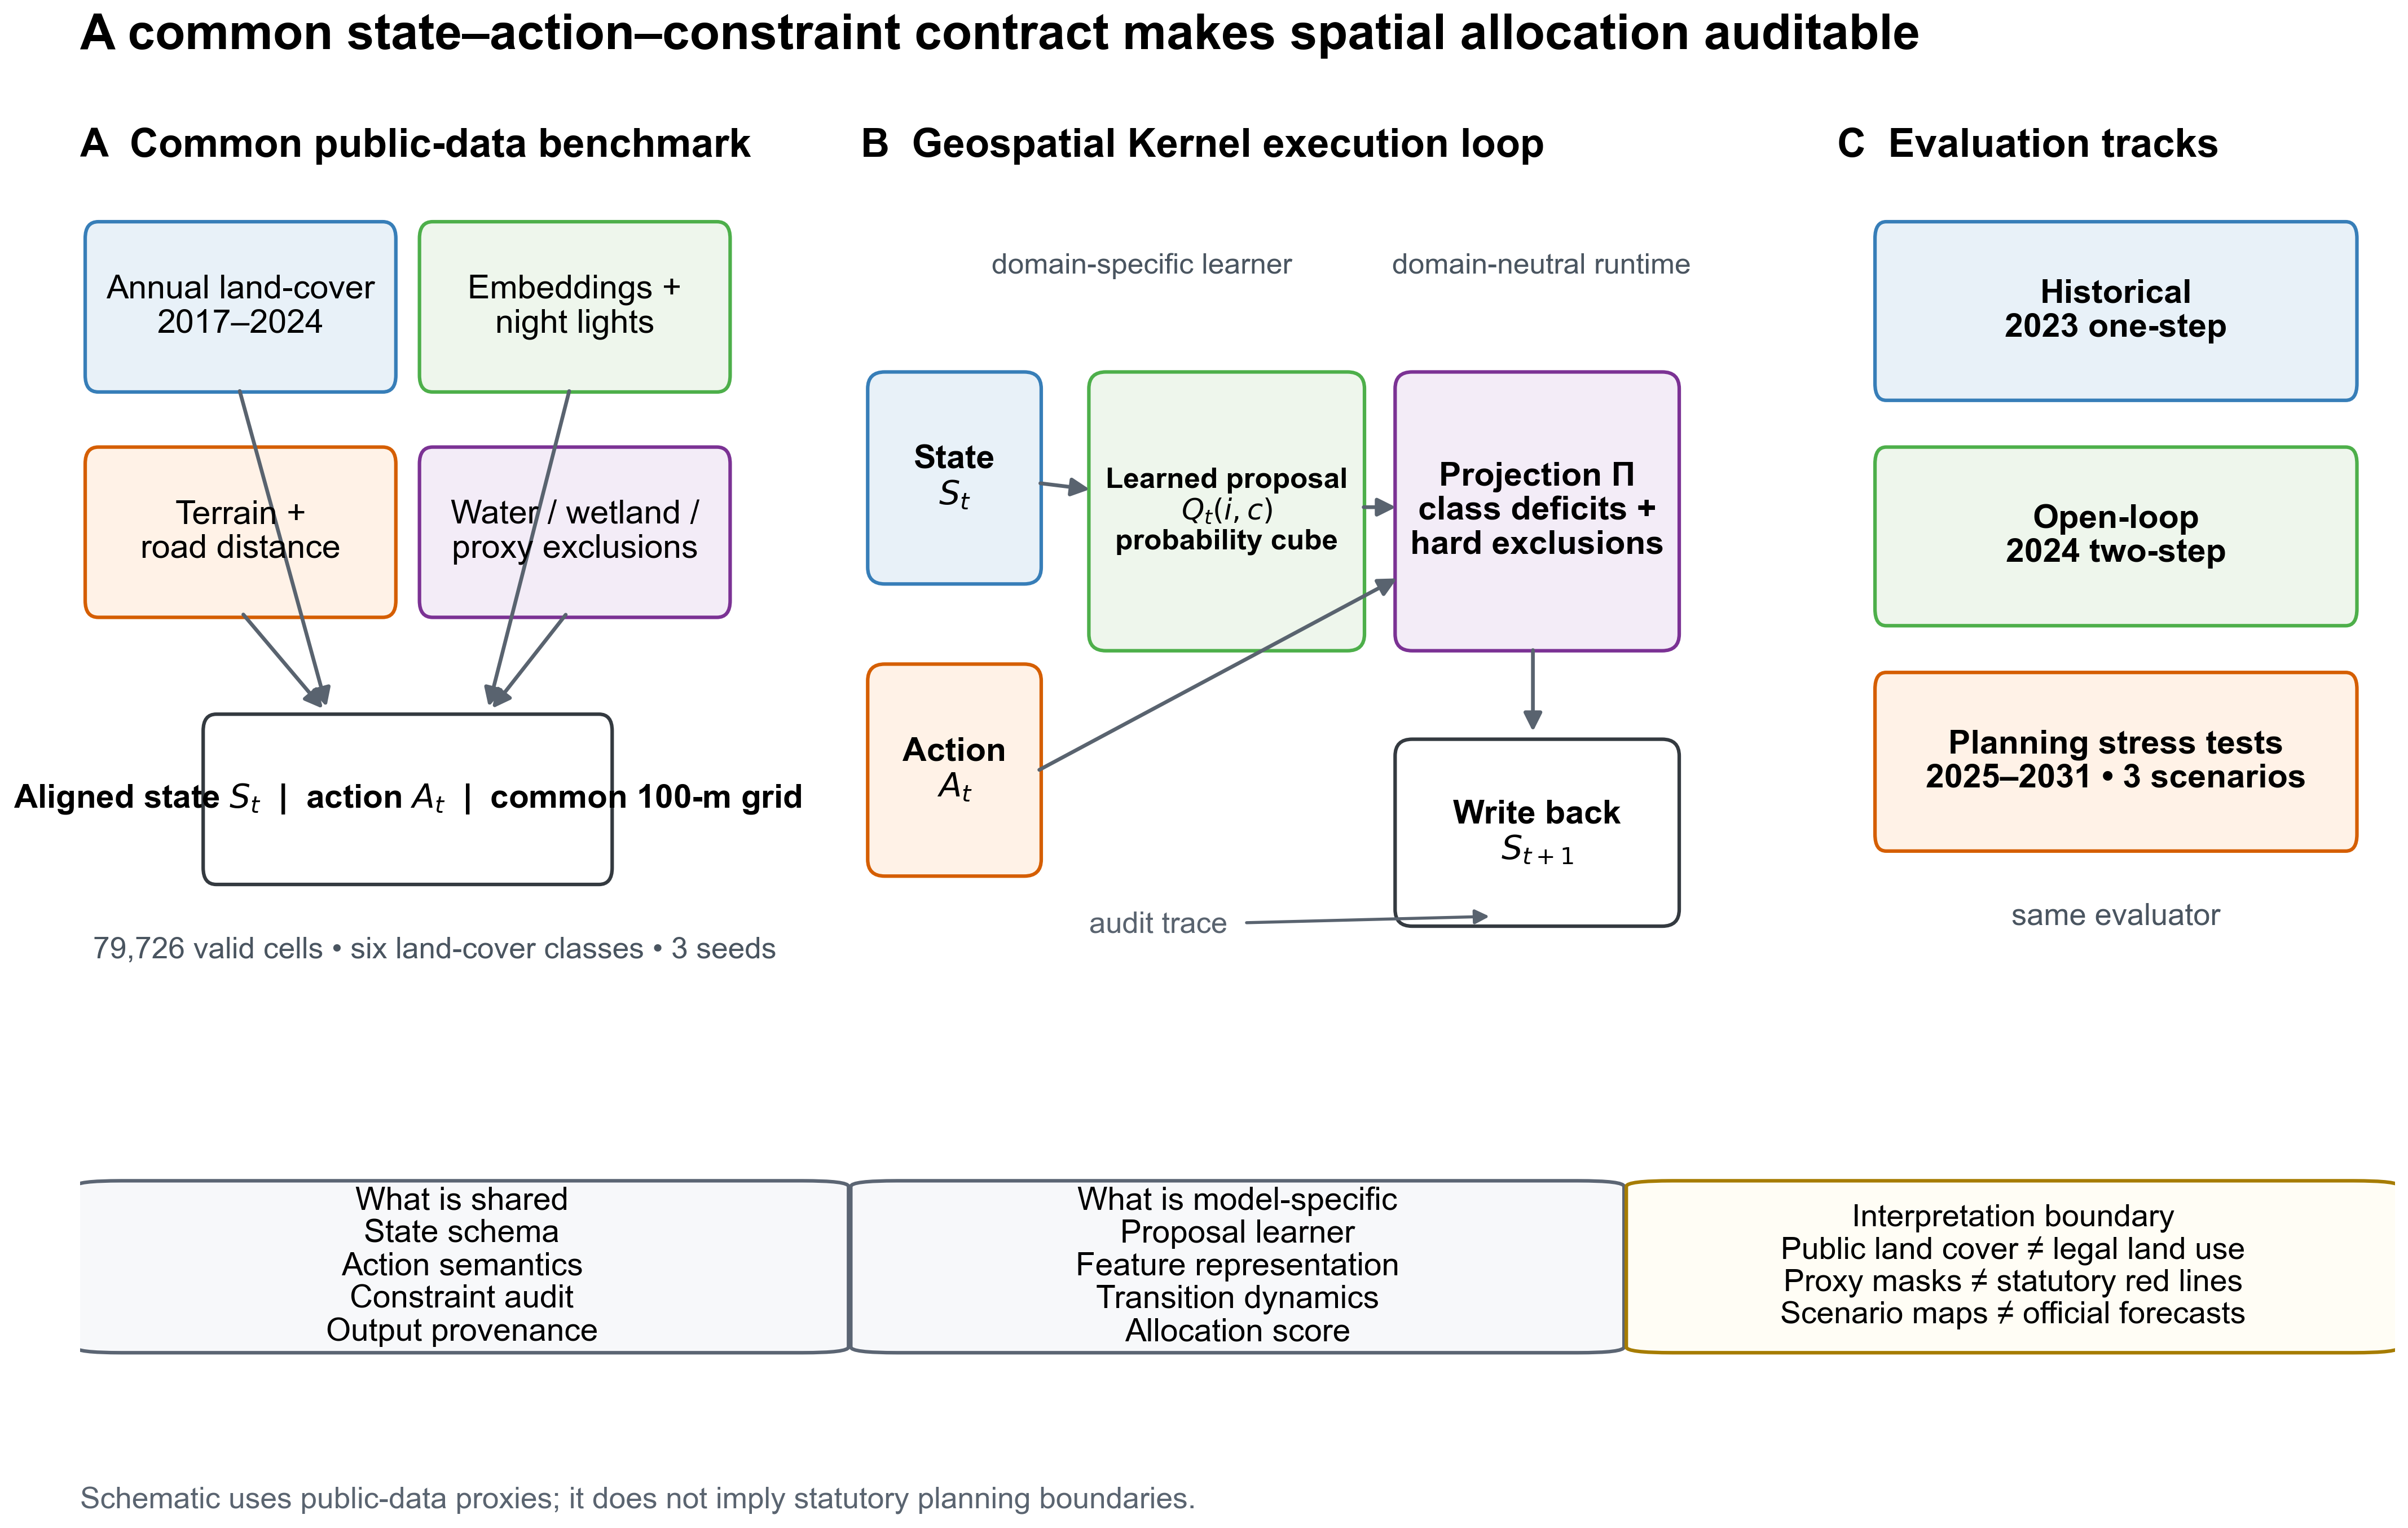
\includegraphics[keepaspectratio,alt={Figure 1: benchmark and execution contract}]{figures/fig01_benchmark_contract.png}}
\caption{Figure 1: benchmark and execution contract}
\end{figure}

\textbf{Figure 1 \textbar{} Benchmark and Geospatial Kernel execution contract.} Public annual land-cover, embedding, night-light, terrain and road layers are aligned to a common 100-m Abu Dhabi grid. Each model receives the same state, action and public proxy exclusions. The Geospatial Kernel exposes a learned proposal, constraint projection and state writeback. Historical, open-loop and planning tracks use one audit contract. The schematic does not imply statutory planning boundaries.

\begin{figure}
\centering
\pandocbounded{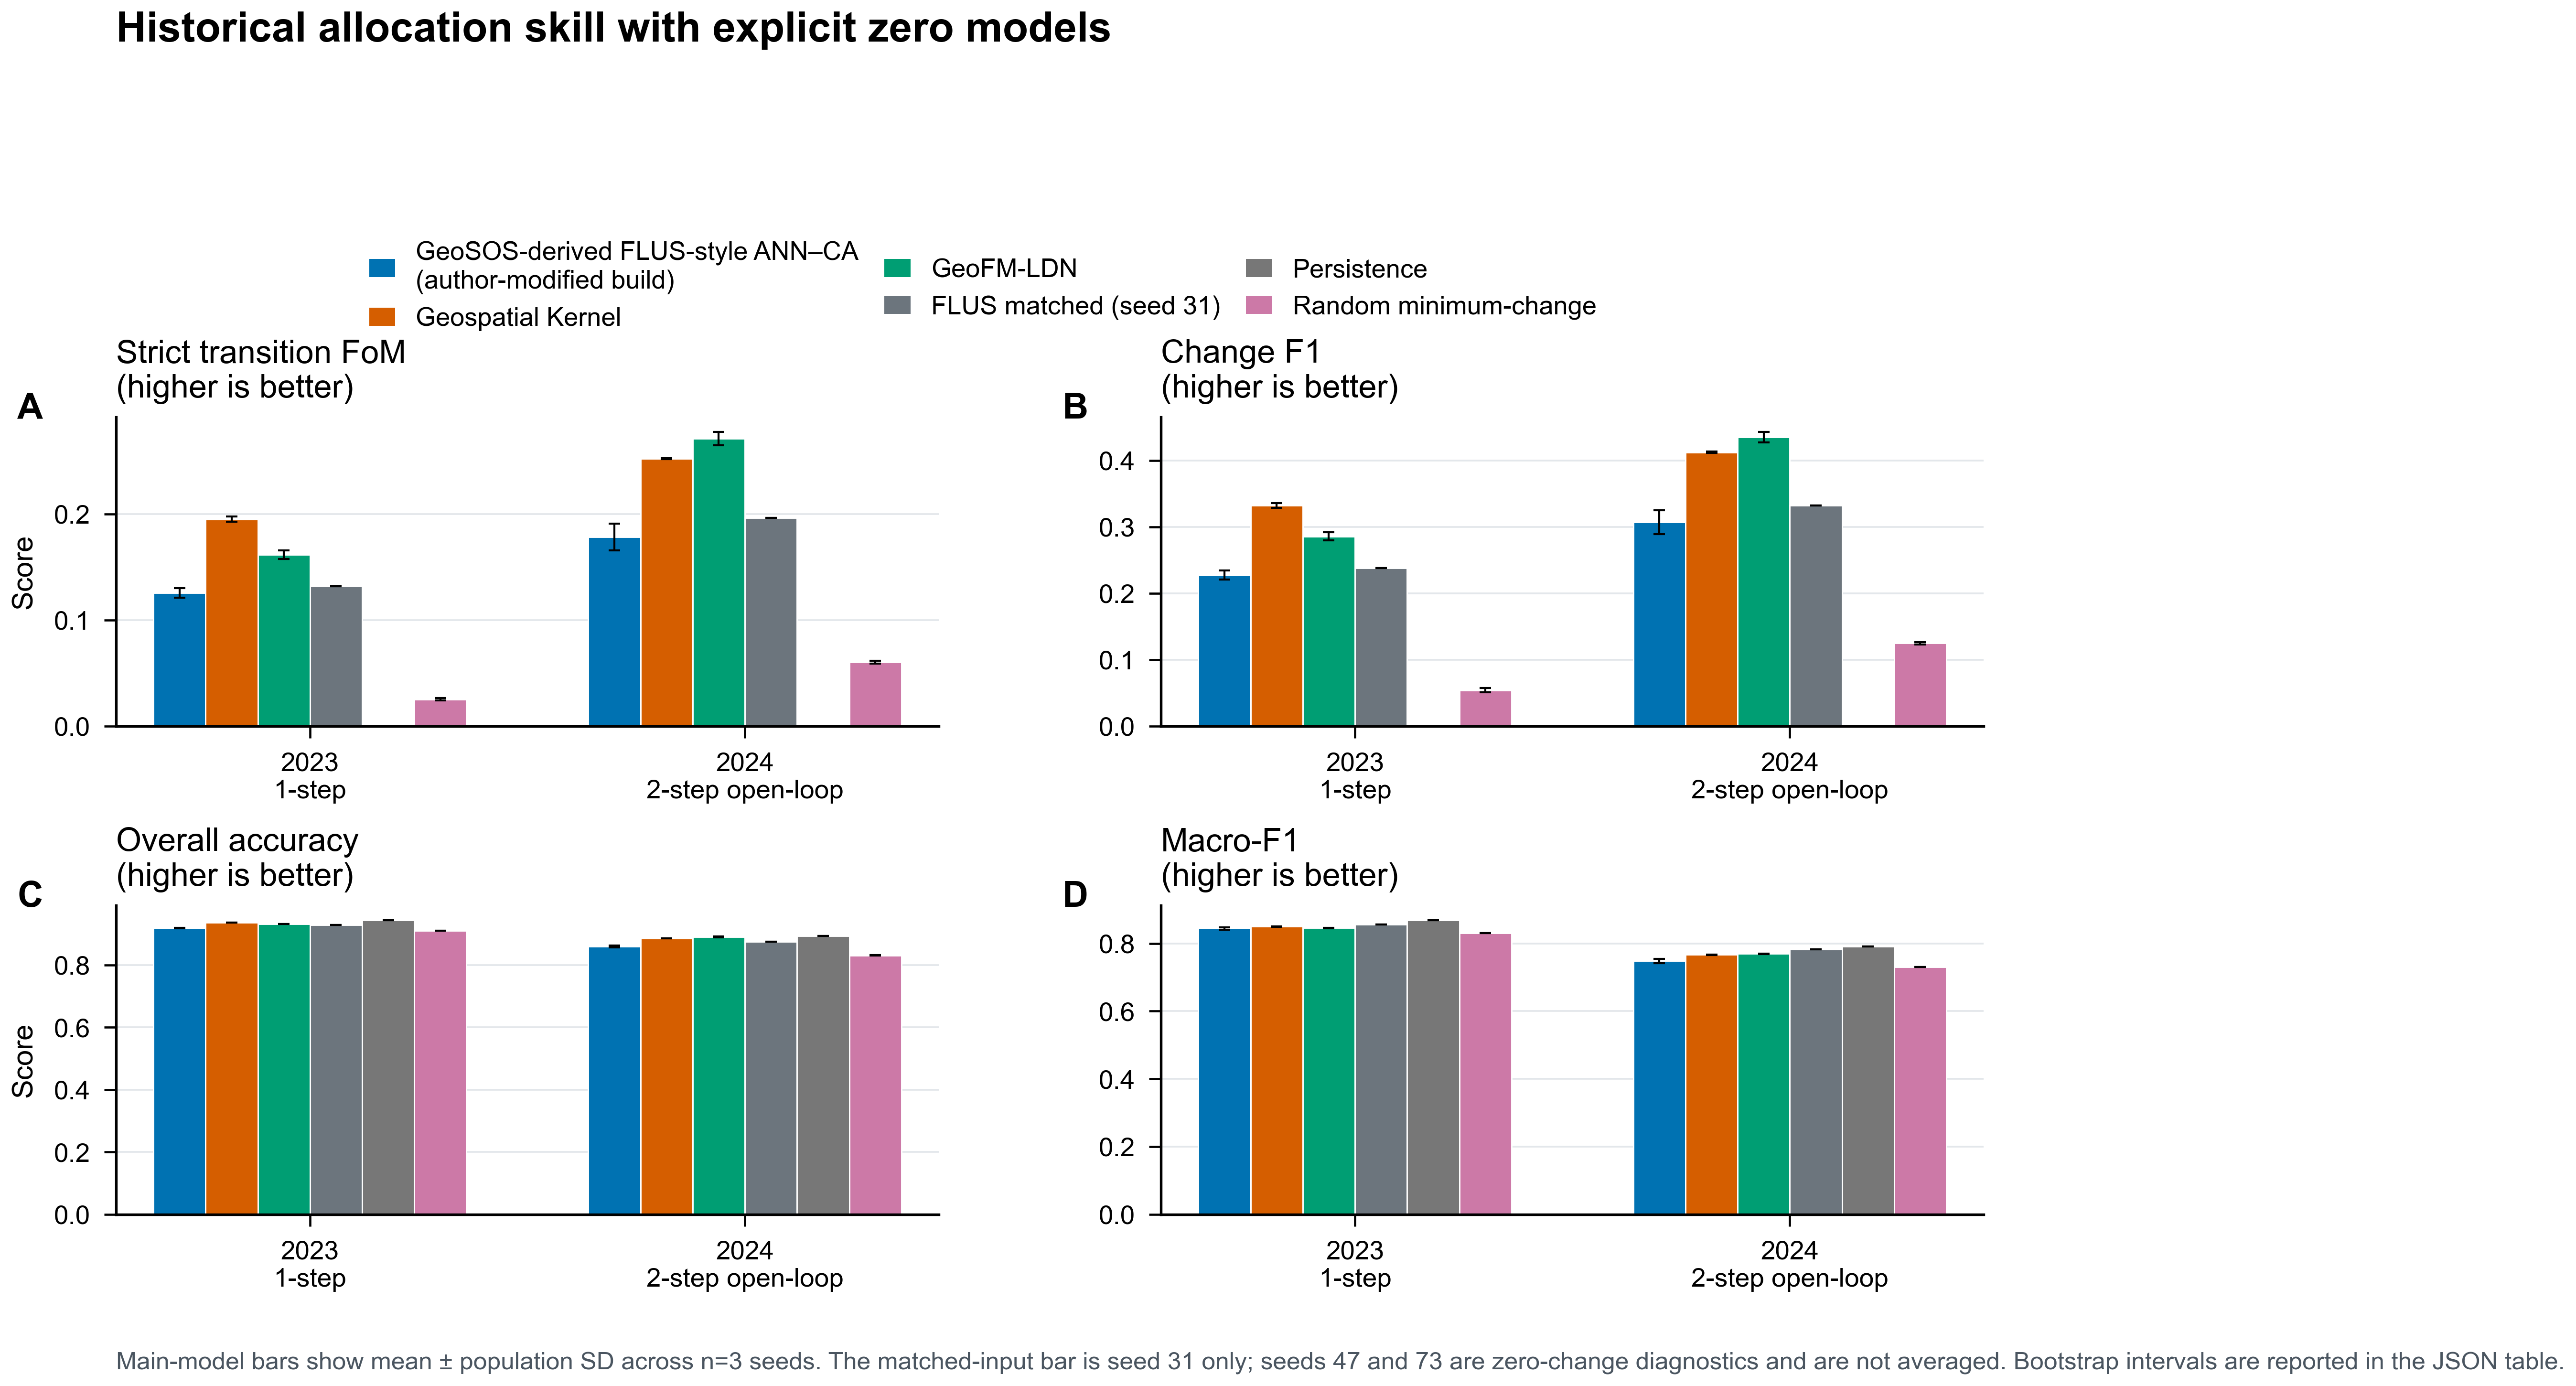
\includegraphics[keepaspectratio,alt={Figure 2: historical allocation skill}]{figures/fig02_historical_validation.png}}
\caption{Figure 2: historical allocation skill}
\end{figure}

\textbf{Figure 2 \textbar{} Historical allocation skill.} Bars show the revised strict multi-class FoM, change F1, overall accuracy and macro-F1 for the 2023 one-step and 2024 two-step open-loop tests, with persistence and random minimum-change controls. Error bars show population standard deviation across the three frozen seeds; paired spatial-block intervals are reported in the machine-readable comparison report.

\begin{figure}
\centering
\pandocbounded{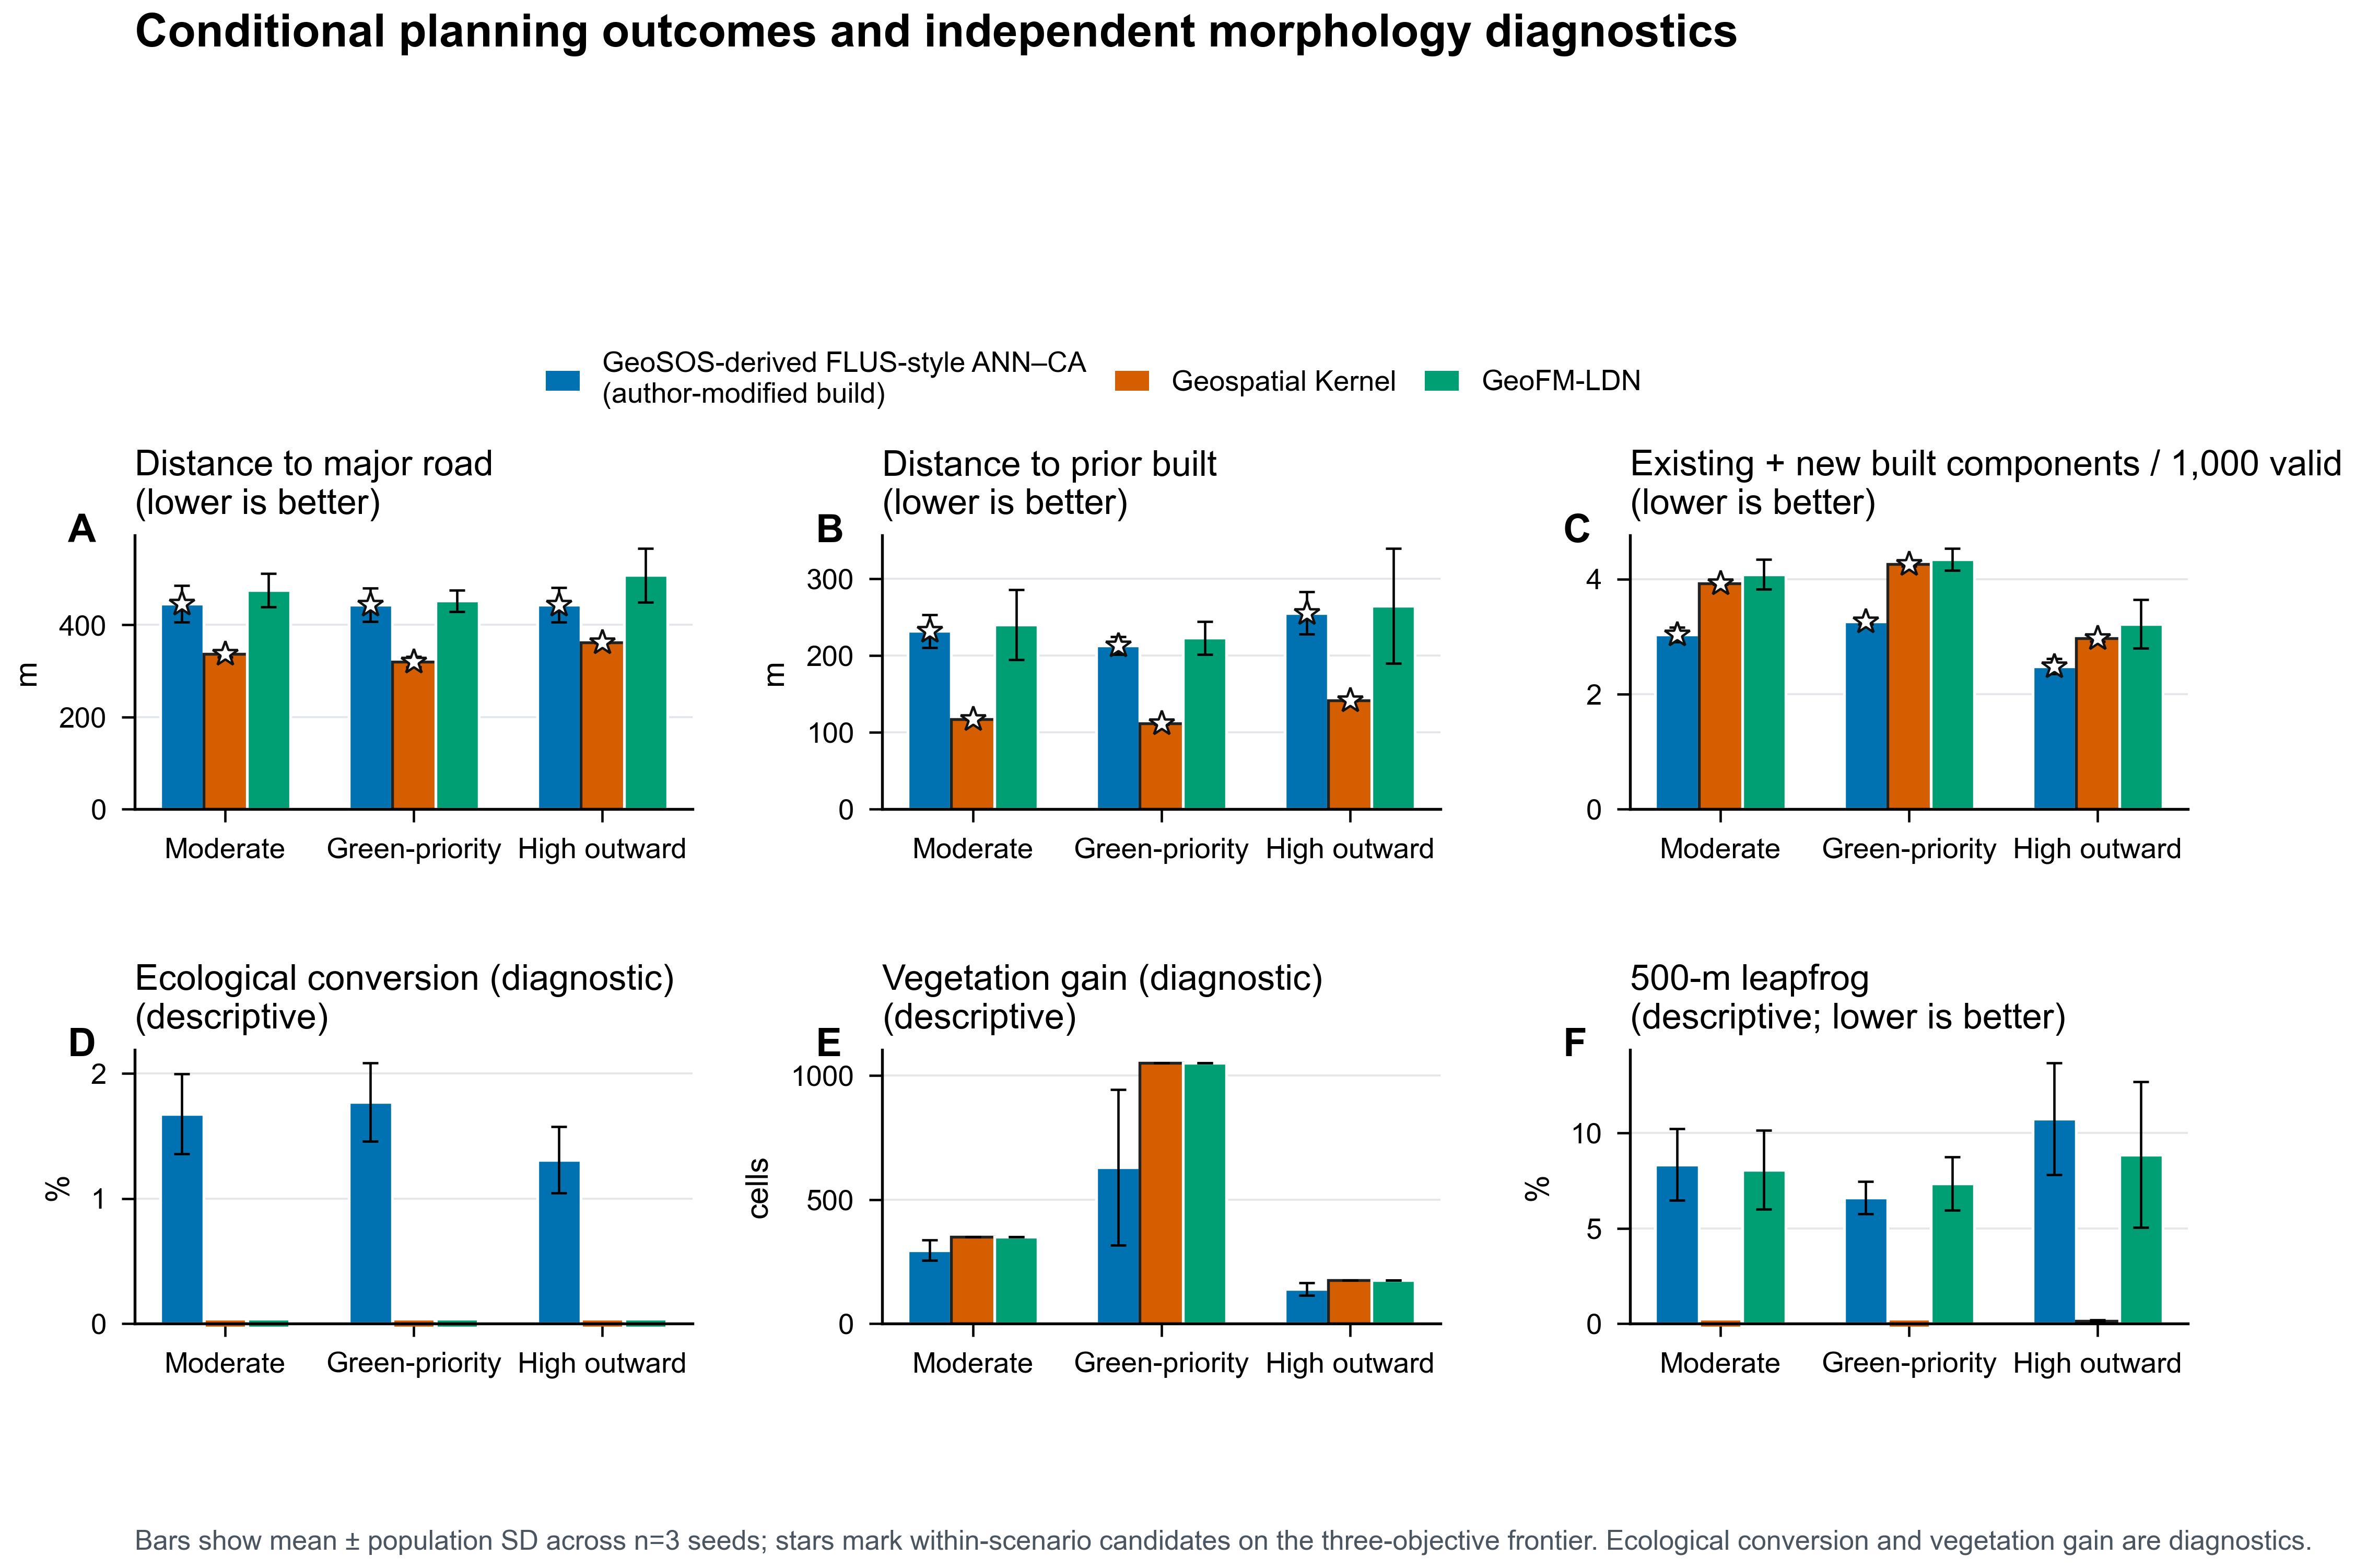
\includegraphics[keepaspectratio,alt={Figure 3: conditional planning objectives}]{figures/fig03_planning_objectives.png}}
\caption{Figure 3: conditional planning objectives}
\end{figure}

\textbf{Figure 3 \textbar{} Conditional planning objectives and morphology diagnostics.} The 2031 outcomes compare the three models under moderate-growth, green-priority- growth and high-outward-growth actions. Panels A--D are the frozen Pareto objectives: distance to major roads, distance to prior built cells, built components per 1,000 valid cells and vegetation gain. Panels E--F are descriptive diagnostics (ecological conversion and 500-m leapfrog rate). Stars mark non-dominated candidates under the four-objective set; bars show means ± population SD across three seeds.

\begin{figure}
\centering
\pandocbounded{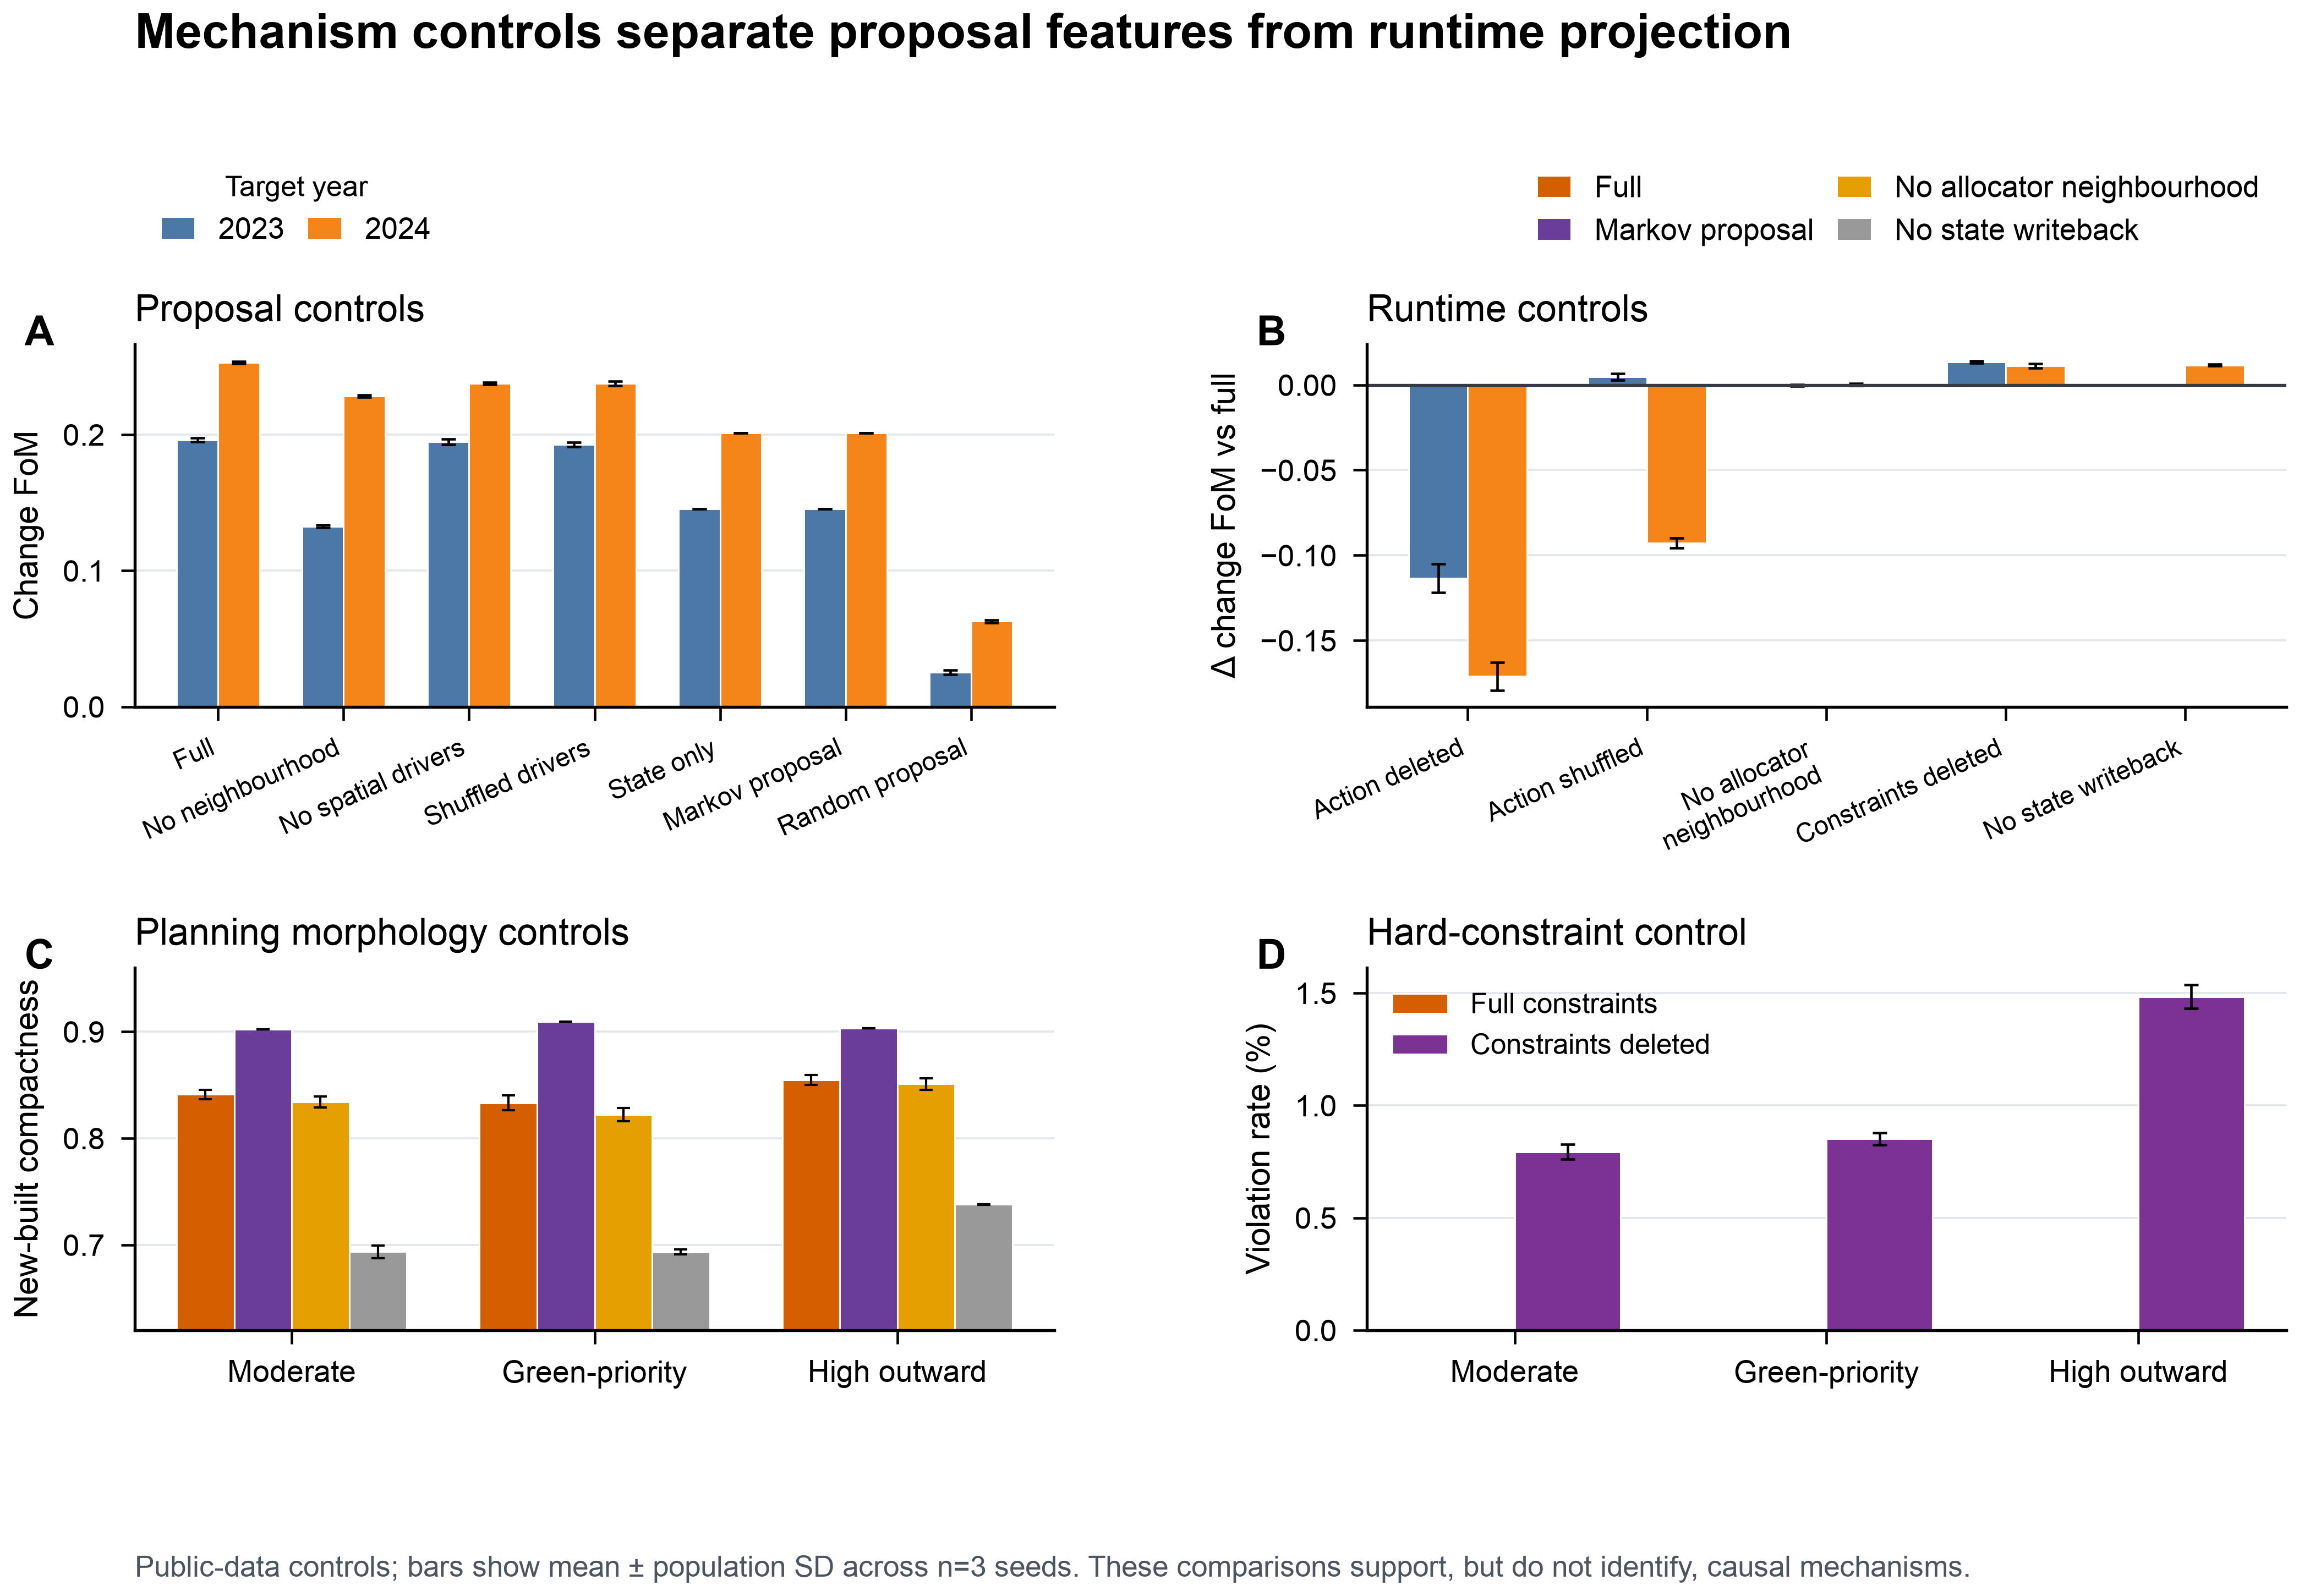
\includegraphics[keepaspectratio,alt={Figure 4: mechanism controls}]{figures/fig04_mechanism_ablation.png}}
\caption{Figure 4: mechanism controls}
\end{figure}

\textbf{Figure 4 \textbar{} Mechanism controls.} Proposal, allocator, action, constraint and writeback controls are compared under the same public-data protocol. Deleting the action lowers historical strict FoM, whereas deleting the hard constraint raises agreement with noisy labels while violating the planning contract. These are diagnostic ablations, not causal policy experiments.

\begin{figure}
\centering
\pandocbounded{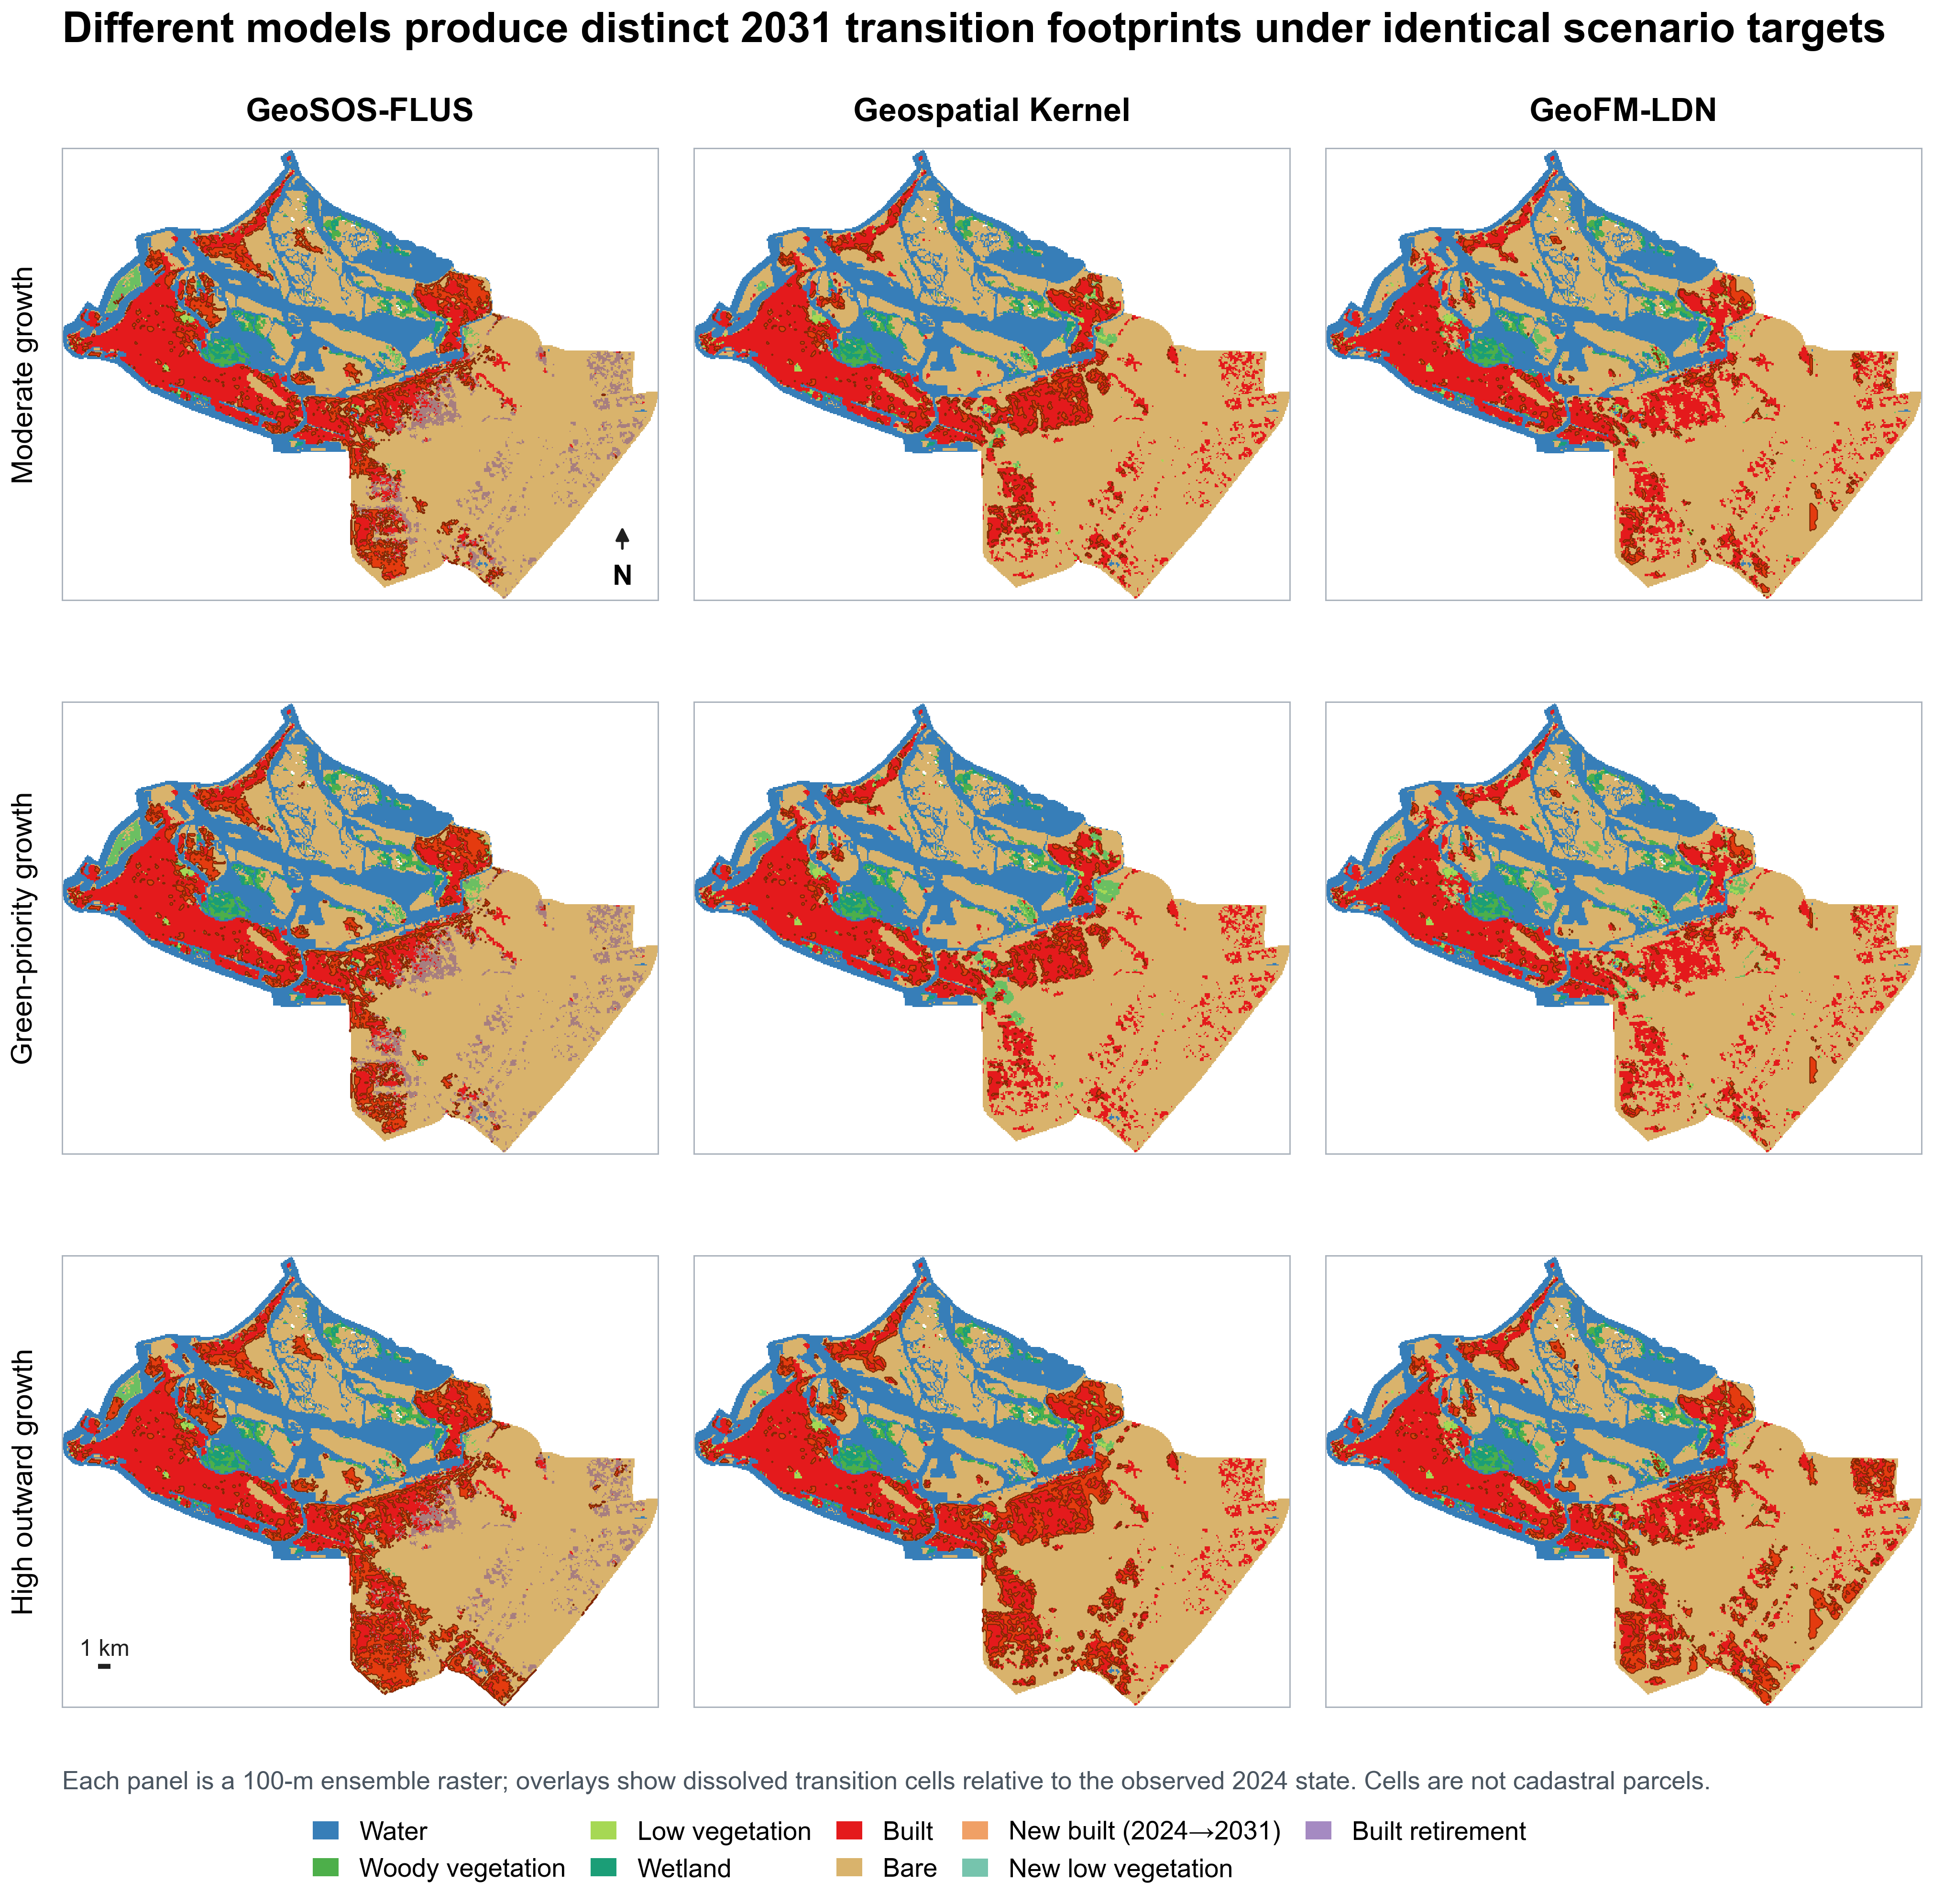
\includegraphics[keepaspectratio,alt={Figure 5: 2031 spatial footprints}]{figures/fig05_planning_maps_2031.png}}
\caption{Figure 5: 2031 spatial footprints}
\end{figure}

\textbf{Figure 5 \textbar{} 2031 spatial footprints.} Each panel is a 100-m ensemble raster relative to the observed 2024 state. Overlays identify newly built, newly low- vegetated and retired-built cells; they are raster-cell change footprints, not cadastral parcels.

\subsection{Supplementary information outline}\label{supplementary-information-outline}

\begin{itemize}
\tightlist
\item
  \textbf{Supplementary Note 1:} Complete data crosswalk, quality metrics and public/proxy status.
\item
  \textbf{Supplementary Note 2:} Kernel runtime schemas, audit fields and adapter boundary.
\item
  \textbf{Supplementary Table S1:} Full 2025--2031 model--scenario objective matrix with per-seed values.
\item
  \textbf{Supplementary Table S2:} Neighbourhood-weight sensitivity at 0, 0.175, 0.35 and 0.7.
\item
  \textbf{Supplementary Table S3:} Raster and vector delivery audit, hashes and layer counts.
\item
  \textbf{Supplementary Figure S1:} Dynamic World confidence and high-confidence change sensitivity.
\item
  \textbf{Supplementary Figure S2:} Historical maps and change-error maps for 2024.
\item
  \textbf{Supplementary Figure S3:} Driver layers and experiment design in English.
\end{itemize}

\begin{center}\rule{0.5\linewidth}{0.5pt}\end{center}

\end{document}
